\section{Datalog and static analysis}

\subsection{Stratified Datalog}

\paragraph{Datalog:}
\begin{itemize}
    \item Declarative logic-programming language.
    \item Useful for expressing recursive queries.
    \item solid formal foundations.
    \item Used in:
    \begin{itemize}
        \item Security Analysis
        \item Network config analysis
        \item Access control
    \end{itemize}{}
\end{itemize}

\paragraph{Datalog atoms:} Datalog consists of a variety of atoms.

\begin{minipage}{0.5\linewidth}
    \centering      
    \def\svgwidth{\linewidth}
    %% Creator: Inkscape inkscape 0.92.4, www.inkscape.org
%% PDF/EPS/PS + LaTeX output extension by Johan Engelen, 2010
%% Accompanies image file 'L3_overflow_exploit.pdf' (pdf, eps, ps)
%%
%% To include the image in your LaTeX document, write
%%   \input{<filename>.pdf_tex}
%%  instead of
%%   \includegraphics{<filename>.pdf}
%% To scale the image, write
%%   \def\svgwidth{<desired width>}
%%   \input{<filename>.pdf_tex}
%%  instead of
%%   \includegraphics[width=<desired width>]{<filename>.pdf}
%%
%% Images with a different path to the parent latex file can
%% be accessed with the `import' package (which may need to be
%% installed) using
%%   \usepackage{import}
%% in the preamble, and then including the image with
%%   \import{<path to file>}{<filename>.pdf_tex}
%% Alternatively, one can specify
%%   \graphicspath{{<path to file>/}}
%% 
%% For more information, please see info/svg-inkscape on CTAN:
%%   http://tug.ctan.org/tex-archive/info/svg-inkscape
%%
\begingroup%
  \makeatletter%
  \providecommand\color[2][]{%
    \errmessage{(Inkscape) Color is used for the text in Inkscape, but the package 'color.sty' is not loaded}%
    \renewcommand\color[2][]{}%
  }%
  \providecommand\transparent[1]{%
    \errmessage{(Inkscape) Transparency is used (non-zero) for the text in Inkscape, but the package 'transparent.sty' is not loaded}%
    \renewcommand\transparent[1]{}%
  }%
  \providecommand\rotatebox[2]{#2}%
  \newcommand*\fsize{\dimexpr\f@size pt\relax}%
  \newcommand*\lineheight[1]{\fontsize{\fsize}{#1\fsize}\selectfont}%
  \ifx\svgwidth\undefined%
    \setlength{\unitlength}{720.00000454bp}%
    \ifx\svgscale\undefined%
      \relax%
    \else%
      \setlength{\unitlength}{\unitlength * \real{\svgscale}}%
    \fi%
  \else%
    \setlength{\unitlength}{\svgwidth}%
  \fi%
  \global\let\svgwidth\undefined%
  \global\let\svgscale\undefined%
  \makeatother%
  \begin{picture}(1,0.75)%
    \lineheight{1}%
    \setlength\tabcolsep{0pt}%
    \put(0,0){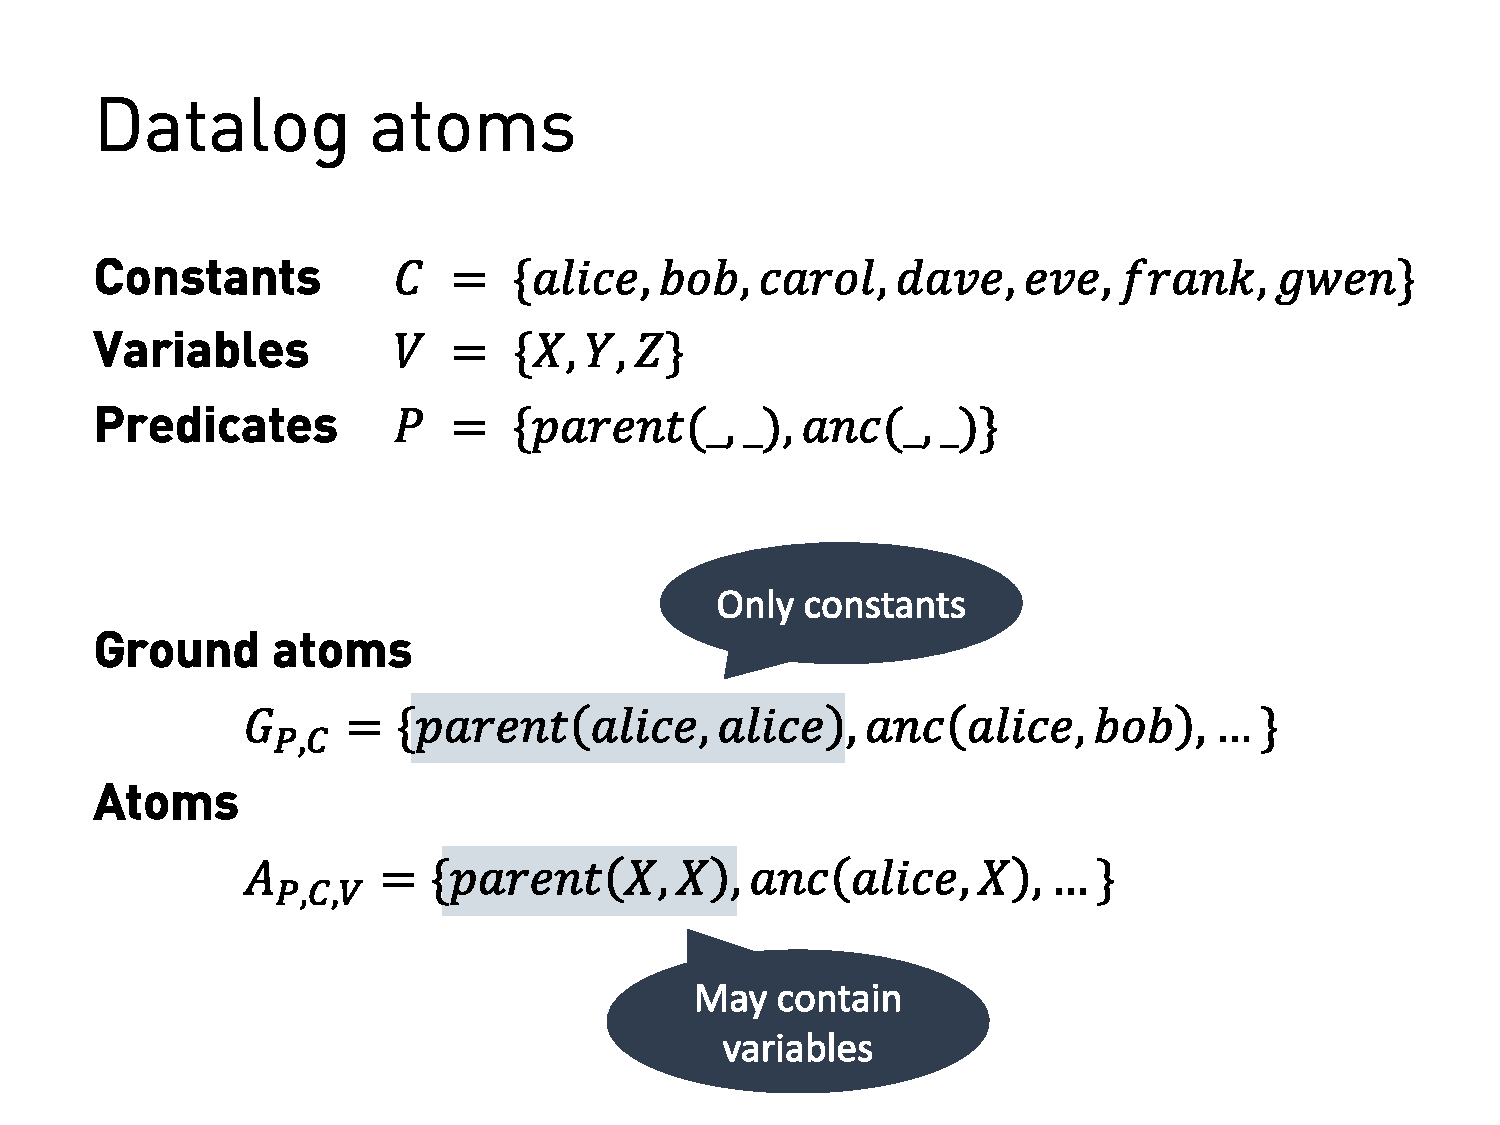
\includegraphics[width=\unitlength,page=1]{Figures/L5_datalog_atoms.pdf}}%
  \end{picture}%
\endgroup%
    
\end{minipage}  
\paragraph{Datalog programs:} 
\begin{itemize}
    \item A set of rules of the form $a \xleftarrow{} l_1,...,l_n$
    \item Where $l_1,...,l_n$ are literals of the form $a$ or $\neg a$
    \item A program is \textcolor{orange}{well-formed} if for any rule, all variables that appear in the head (left of arrow) also appear in the body (right of arrow). Plus the variables in the head are not allowed to be negated.
    \item Predicates are not allowed to by cyclic and appear in negative literals.
    \item A program is \textcolor{orange}{positive} if its rules do not contain negative literals.
    \item The semantics of a positive Datalog program P is the least-fixed point of it.
    \item For any positive Datalog program the consequence operator $T_P$ is \textcolor{orange}{monotone}, but not for programs with negation.
\end{itemize}{}

\paragraph{Consequence Operator $T_P / \jmath$:}
\begin{itemize}
    \item \textcolor{blue}{$T_p(I) = \{\sigma(a) | a \xleftarrow{} l_1,...,l_n \in P, \exists \sigma : \forall i \in [1,...,n]: I \vdash \sigma(l_i)\}$}
    \item[] where \textcolor{blue}{$I \vdash l_i$ if $l_i = a$ and $a \in I$}
    \item[] and \textcolor{blue}{$I \vdash l_i$ if $l_i = \neg a$ and $a \notin I$}
    \item Note that ($\jmath, \subseteq, \cup, \cap$) is a complete lattice.
    \item \textbf{Least-fixed point $lfp_{T_P}$} can be computed by iteratively applying the consequene operator until reaching a fixed-point.
\end{itemize}{}

\paragraph{Stratified Datalog programs:}
\begin{itemize}
    \item Same predicate rules in one stratum.
    \item Negated predicate defined in lower stratum.
    \item Positive predicates defined in curren or lower stratum.
    \item[$\xrightarrow{}$] For each stratum, compute the lfp that contains the lfp of the previous stratum.
\end{itemize}{}

\begin{minipage}{0.5\linewidth}
    \centering      
    \def\svgwidth{\linewidth}
    %% Creator: Inkscape 1.0 (4035a4fb49, 2020-05-01), www.inkscape.org
%% PDF/EPS/PS + LaTeX output extension by Johan Engelen, 2010
%% Accompanies image file 'L5_stratified_datalog.pdf' (pdf, eps, ps)
%%
%% To include the image in your LaTeX document, write
%%   \input{<filename>.pdf_tex}
%%  instead of
%%   \includegraphics{<filename>.pdf}
%% To scale the image, write
%%   \def\svgwidth{<desired width>}
%%   \input{<filename>.pdf_tex}
%%  instead of
%%   \includegraphics[width=<desired width>]{<filename>.pdf}
%%
%% Images with a different path to the parent latex file can
%% be accessed with the `import' package (which may need to be
%% installed) using
%%   \usepackage{import}
%% in the preamble, and then including the image with
%%   \import{<path to file>}{<filename>.pdf_tex}
%% Alternatively, one can specify
%%   \graphicspath{{<path to file>/}}
%% 
%% For more information, please see info/svg-inkscape on CTAN:
%%   http://tug.ctan.org/tex-archive/info/svg-inkscape
%%
\begingroup%
  \makeatletter%
  \providecommand\color[2][]{%
    \errmessage{(Inkscape) Color is used for the text in Inkscape, but the package 'color.sty' is not loaded}%
    \renewcommand\color[2][]{}%
  }%
  \providecommand\transparent[1]{%
    \errmessage{(Inkscape) Transparency is used (non-zero) for the text in Inkscape, but the package 'transparent.sty' is not loaded}%
    \renewcommand\transparent[1]{}%
  }%
  \providecommand\rotatebox[2]{#2}%
  \newcommand*\fsize{\dimexpr\f@size pt\relax}%
  \newcommand*\lineheight[1]{\fontsize{\fsize}{#1\fsize}\selectfont}%
  \ifx\svgwidth\undefined%
    \setlength{\unitlength}{720.00000454bp}%
    \ifx\svgscale\undefined%
      \relax%
    \else%
      \setlength{\unitlength}{\unitlength * \real{\svgscale}}%
    \fi%
  \else%
    \setlength{\unitlength}{\svgwidth}%
  \fi%
  \global\let\svgwidth\undefined%
  \global\let\svgscale\undefined%
  \makeatother%
  \begin{picture}(1,0.75)%
    \lineheight{1}%
    \setlength\tabcolsep{0pt}%
    \put(0,0){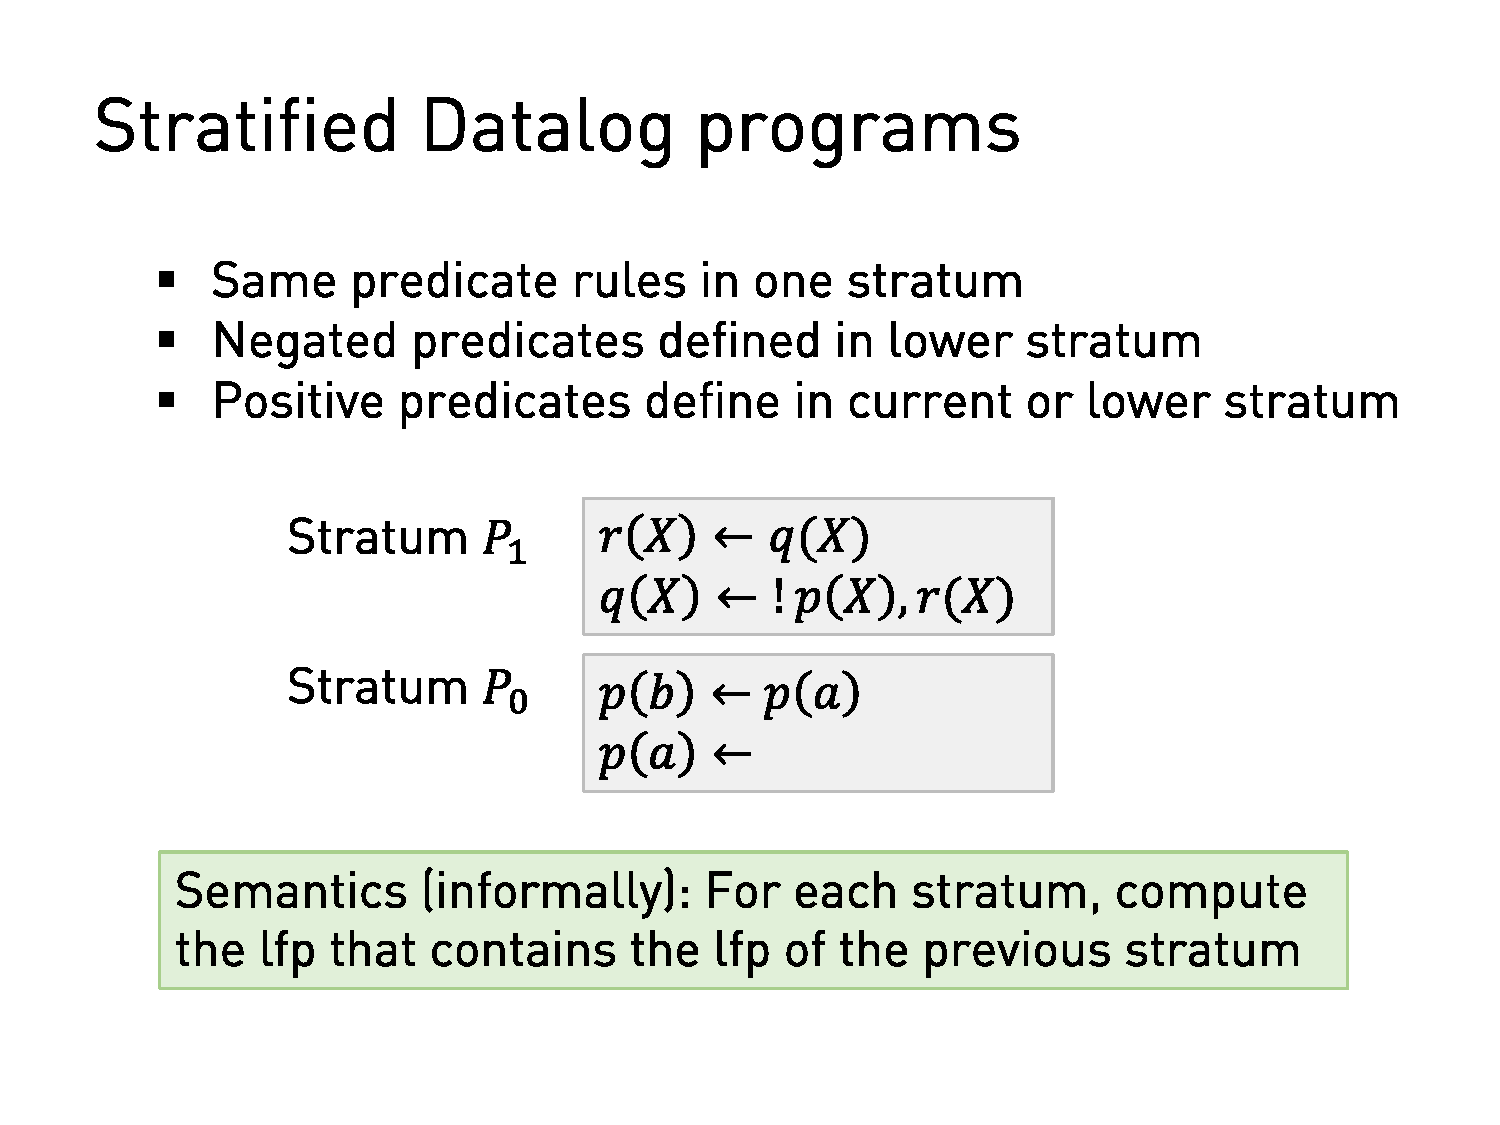
\includegraphics[width=\unitlength,page=1]{L5_stratified_datalog.pdf}}%
  \end{picture}%
\endgroup%    
\end{minipage} 

\subsection{Static analysis with Datalog}

\paragraph{Effective callback freedom EECF:} A contract is EECF if for any execution with external callbacks there exists an equivalent execution without external callbacks (which starts in the same state and reaches the same final state).
\begin{itemize}
    \item[$\xrightarrow{}$] In practice, developers enforce the following security property: \textcolor{red}{Do not perform any stat changes after calls to external contracts.}
\end{itemize}{}

\paragraph{Checking security properties:}
\begin{itemize}
    \item Usually we cannot automatically find all calls where a certain property does not hold, because smart contracts are Turing-complete.
    \item However, when contracts violate/satisfy a security property they often violate/satisfy a simpler property. (E.g. instead of EECF check if there are writes after call.value())
\end{itemize}{}

\paragraph{Securify: } v2.0

\begin{minipage}{0.9\linewidth}
    \centering      
    \def\svgwidth{\linewidth}
    %% Creator: Inkscape inkscape 0.92.4, www.inkscape.org
%% PDF/EPS/PS + LaTeX output extension by Johan Engelen, 2010
%% Accompanies image file 'L5_securify.pdf' (pdf, eps, ps)
%%
%% To include the image in your LaTeX document, write
%%   \input{<filename>.pdf_tex}
%%  instead of
%%   \includegraphics{<filename>.pdf}
%% To scale the image, write
%%   \def\svgwidth{<desired width>}
%%   \input{<filename>.pdf_tex}
%%  instead of
%%   \includegraphics[width=<desired width>]{<filename>.pdf}
%%
%% Images with a different path to the parent latex file can
%% be accessed with the `import' package (which may need to be
%% installed) using
%%   \usepackage{import}
%% in the preamble, and then including the image with
%%   \import{<path to file>}{<filename>.pdf_tex}
%% Alternatively, one can specify
%%   \graphicspath{{<path to file>/}}
%% 
%% For more information, please see info/svg-inkscape on CTAN:
%%   http://tug.ctan.org/tex-archive/info/svg-inkscape
%%
\begingroup%
  \makeatletter%
  \providecommand\color[2][]{%
    \errmessage{(Inkscape) Color is used for the text in Inkscape, but the package 'color.sty' is not loaded}%
    \renewcommand\color[2][]{}%
  }%
  \providecommand\transparent[1]{%
    \errmessage{(Inkscape) Transparency is used (non-zero) for the text in Inkscape, but the package 'transparent.sty' is not loaded}%
    \renewcommand\transparent[1]{}%
  }%
  \providecommand\rotatebox[2]{#2}%
  \newcommand*\fsize{\dimexpr\f@size pt\relax}%
  \newcommand*\lineheight[1]{\fontsize{\fsize}{#1\fsize}\selectfont}%
  \ifx\svgwidth\undefined%
    \setlength{\unitlength}{720.00000454bp}%
    \ifx\svgscale\undefined%
      \relax%
    \else%
      \setlength{\unitlength}{\unitlength * \real{\svgscale}}%
    \fi%
  \else%
    \setlength{\unitlength}{\svgwidth}%
  \fi%
  \global\let\svgwidth\undefined%
  \global\let\svgscale\undefined%
  \makeatother%
  \begin{picture}(1,0.75)%
    \lineheight{1}%
    \setlength\tabcolsep{0pt}%
    \put(0,0){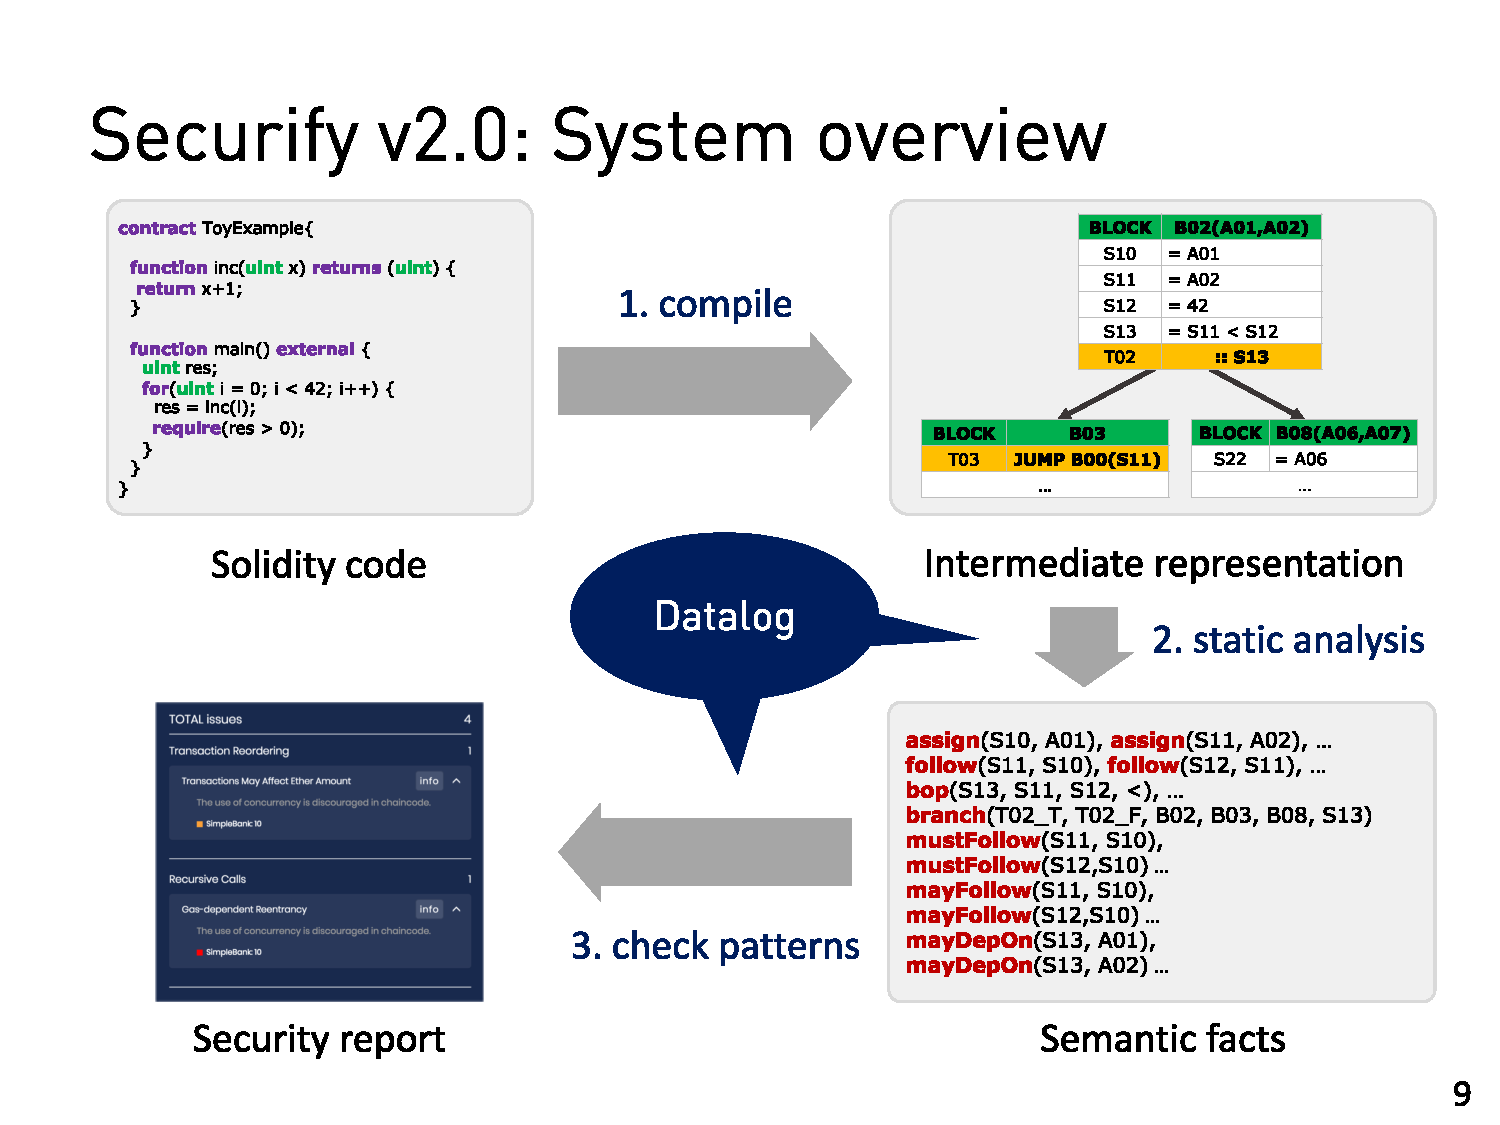
\includegraphics[width=\unitlength,page=1]{Figures/L5_securify.pdf}}%
  \end{picture}%
\endgroup%
    
\end{minipage}

\begin{itemize}
    \item Securify compiles Solidity to IR (Intermediate Representation)
    \item Bytecode is too low-level and lacks semantic information (No function boundaries, no storage model)
    \item Source code (Solidity) is too rich/changes often. This leads to a complex analysis.
    \item \textbf{Basic blocks: }
    \begin{itemize}
        \item Sequence of statements without branching.
        \item Take Arguments
        \item All variables are in single static assignment (SSA) form.
        \item End with a transfer to next blocks
    \end{itemize}{}
    \item \textbf{Transfers:} Goto, Jumps, Branches. Args and return values passed to next block
    \item \textbf{Statements:} 
    \begin{itemize}
        \item Static Single Assignment (SSA): each variable is treated as a variable that stores the statement's result.
        \item Three address form: t0 = t1 op t2
    \end{itemize}{}
\end{itemize}{}

\paragraph{Securify: Inferring semantic facts}
\begin{itemize}
    \item Scalable inference of semantic facts using Datalog.
    \item IR $\xrightarrow{}$ Datalog input $\xrightarrow{}$ Datalog fixpoint.
\end{itemize}{}

\begin{minipage}{0.9\linewidth}
    \centering      
    \def\svgwidth{\linewidth}
    %% Creator: Inkscape inkscape 0.92.4, www.inkscape.org
%% PDF/EPS/PS + LaTeX output extension by Johan Engelen, 2010
%% Accompanies image file 'L5_semantic_facts.pdf' (pdf, eps, ps)
%%
%% To include the image in your LaTeX document, write
%%   \input{<filename>.pdf_tex}
%%  instead of
%%   \includegraphics{<filename>.pdf}
%% To scale the image, write
%%   \def\svgwidth{<desired width>}
%%   \input{<filename>.pdf_tex}
%%  instead of
%%   \includegraphics[width=<desired width>]{<filename>.pdf}
%%
%% Images with a different path to the parent latex file can
%% be accessed with the `import' package (which may need to be
%% installed) using
%%   \usepackage{import}
%% in the preamble, and then including the image with
%%   \import{<path to file>}{<filename>.pdf_tex}
%% Alternatively, one can specify
%%   \graphicspath{{<path to file>/}}
%% 
%% For more information, please see info/svg-inkscape on CTAN:
%%   http://tug.ctan.org/tex-archive/info/svg-inkscape
%%
\begingroup%
  \makeatletter%
  \providecommand\color[2][]{%
    \errmessage{(Inkscape) Color is used for the text in Inkscape, but the package 'color.sty' is not loaded}%
    \renewcommand\color[2][]{}%
  }%
  \providecommand\transparent[1]{%
    \errmessage{(Inkscape) Transparency is used (non-zero) for the text in Inkscape, but the package 'transparent.sty' is not loaded}%
    \renewcommand\transparent[1]{}%
  }%
  \providecommand\rotatebox[2]{#2}%
  \newcommand*\fsize{\dimexpr\f@size pt\relax}%
  \newcommand*\lineheight[1]{\fontsize{\fsize}{#1\fsize}\selectfont}%
  \ifx\svgwidth\undefined%
    \setlength{\unitlength}{600.3286781bp}%
    \ifx\svgscale\undefined%
      \relax%
    \else%
      \setlength{\unitlength}{\unitlength * \real{\svgscale}}%
    \fi%
  \else%
    \setlength{\unitlength}{\svgwidth}%
  \fi%
  \global\let\svgwidth\undefined%
  \global\let\svgscale\undefined%
  \makeatother%
  \begin{picture}(1,0.54994243)%
    \lineheight{1}%
    \setlength\tabcolsep{0pt}%
    \put(0,0){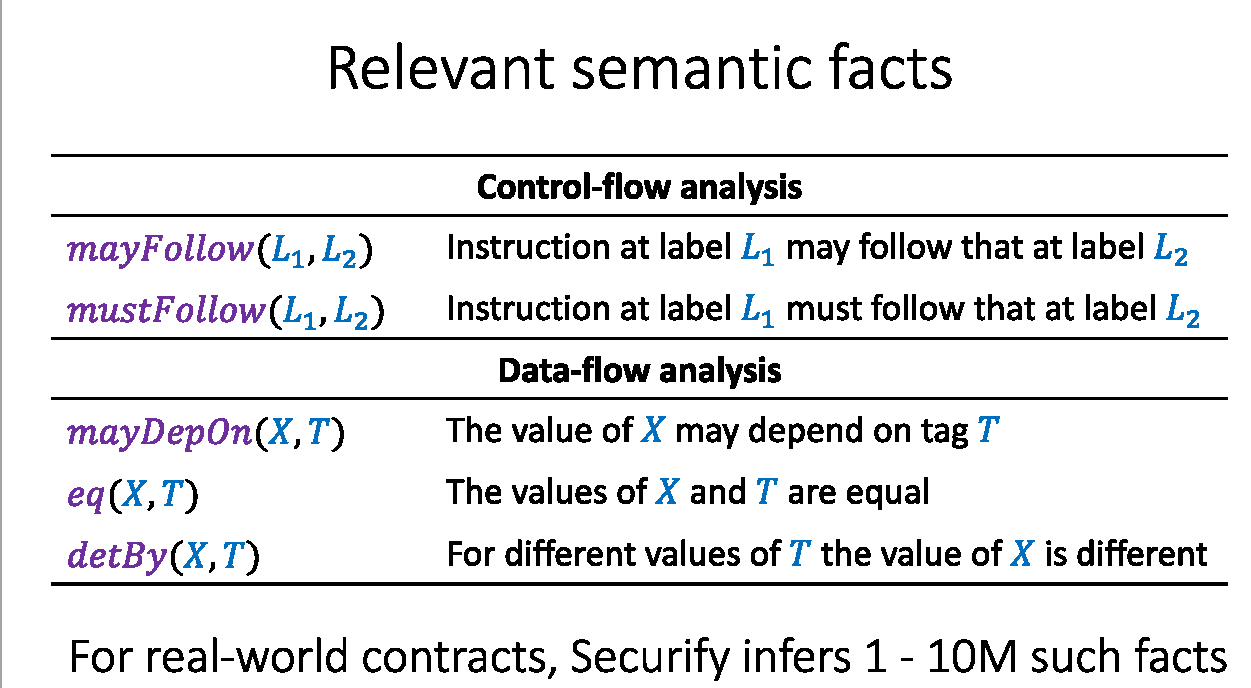
\includegraphics[width=\unitlength,page=1]{Figures/L5_semantic_facts.pdf}}%
  \end{picture}%
\endgroup%
    
\end{minipage}

\paragraph{Taint analysis:} 
\begin{itemize}
    \item Taint analysis is a popular method which consists to check which variables can be modified by the user input. All user input can be dangerous if they aren't properly checked.
    \item \textbf{Call-site sensitivity: }Function arguments are tainted as they are controlled by the user $\rightarrow$ \textcolor{blue}{\texttt{mayDepOn(arguments, tainted)}}
    \item Context tracks a bounded history of the most recent function calls (e.g. context = [func1, func2,...]). $\rightarrow$  \textcolor{blue}{\texttt{mayDepOn(context, variable, tainted)}}
\end{itemize}{}

\paragraph{Security patterns language:}
\begin{itemize}
    \item A security pattern is a logical formula over semantic predicates e.g:\\
    $\varphi = mayDepOn(X,Y) | mustFollow(L,L) | \neg \alpha | ...$
    \item We need to convert a Security property e.g. "No state changes after call instructions" to a suitable violation pattern for securify.
    \item Securify then creates a Security report, where all unsafe calls are reported as either violations or warnings.
\end{itemize}{}

\paragraph{Benefits of static analysis using Datalog:}
\begin{itemize}
    \item Declarative (concise spec of the analysis)
    \item Modular (can merge the rules of multiple analyses)
    \item Scalable (can leverage existing Datalog solvers)
\end{itemize}{}